\chapter{Proposal}\label{cap_proposal}

This chapter demonstrates how to write strictly vanilla LaTeX so that the conversion tool builds a beautiful, native LyX interface. 

\section{Basic Text and Lists}
\label{sec:lists}

When creating lists, ensure there is an empty line before and after the environment. Do not use inline arguments like \texttt{[label=...]} inside the text body.

\begin{itemize}
\item First essential item for the dissertation.
\item Second essential item, showing a clean bullet.
\end{itemize}

\begin{enumerate}
\item First numbered step in the methodology.
\item Second numbered step.
\end{enumerate}

\section{Cross-References and Citations}
\label{sec:cross_ref}

To reference figures and tables within the text, use standard reference commands so LyX maps them to native cross-reference links. For example, see the single image in Figure~\ref{fig:single}, or the side-by-side images in Figure~\ref{fig:side_a} and Figure~\ref{fig:side_b}. The data is summarized in Table~\ref{tab:results}.

For citations in the abnTeX2 format, use the standard citation commands. This is an example of an indirect citation at the end of a sentence \cite{araujo2012}. On the other hand, as mentioned by \citeonline{araujo2012}, you can also integrate direct citations naturally into the flow of your text.

\section{Mathematical Equations}
\label{sec:math}

Standard math imports perfectly into LyX's native formula editor.

This is an inline equation: $E = mc^2$, which will appear naturally in the text. For display equations, use the standard equation environment:

\begin{equation}
\label{eq:fourier}
f(x) = a_0 + \sum_{n=1}^{\infty} \left( a_n \cos\left(\frac{n\pi x}{L}\right) + b_n \sin\left(\frac{n\pi x}{L}\right) \right)
\end{equation}

\section{Figures and Minipages}
\label{sec:figures}

Wrap the image in a \texttt{centering} environment (instead of \texttt{center}) to prevent LyX ERT boxes while avoiding extra vertical spacing in the final PDF.

\begin{figure}[htbp]
\begin{centering}
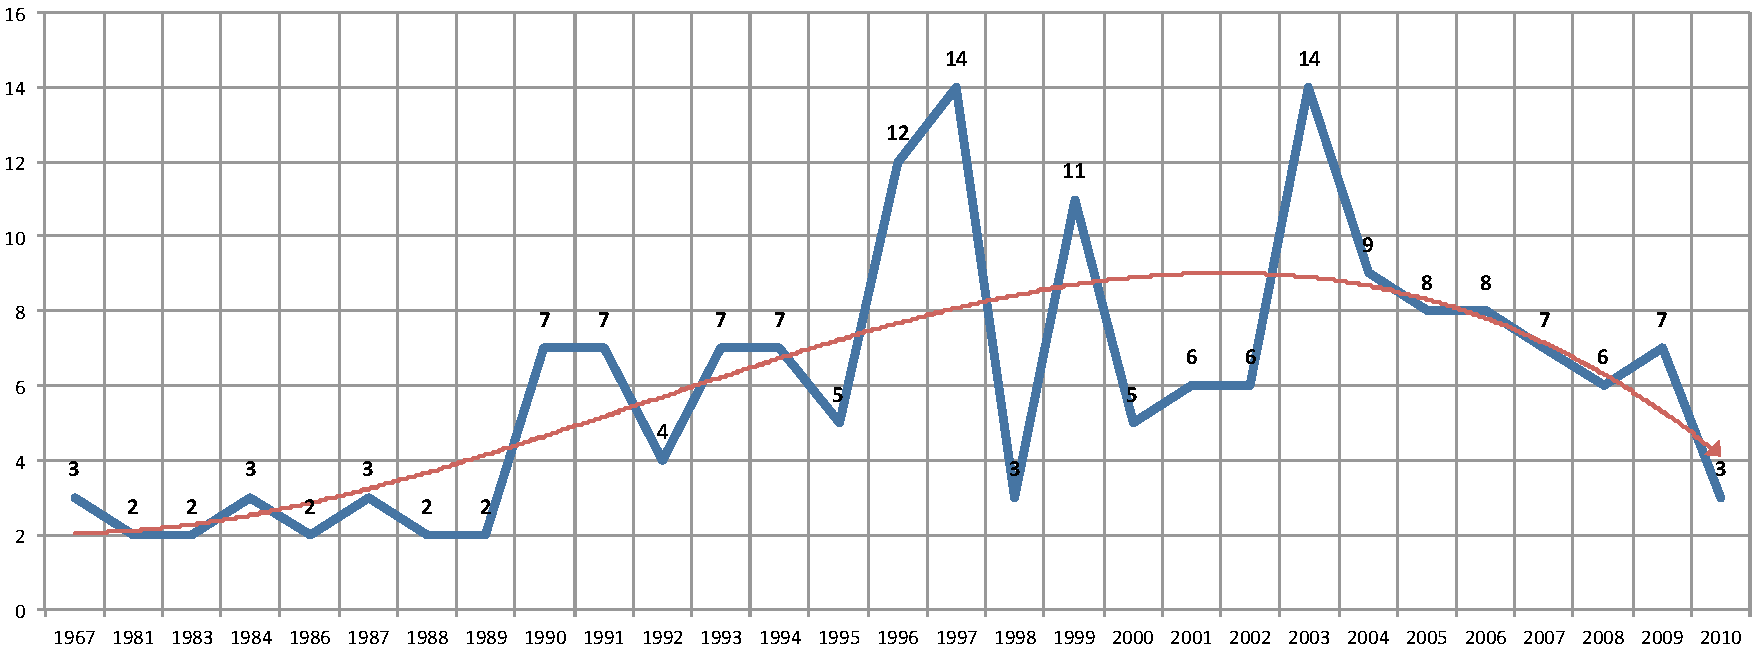
\includegraphics[width=0.6\textwidth]{figuras/abntex2-modelo-img-grafico.pdf}
\par\end{centering}
\caption{A perfectly formatted single figure.\label{fig:single}}

\legend{Fonte: Produzido pelos autores.}
\end{figure}

To place two figures side-by-side, use \texttt{minipage} blocks directly inside the figure environment. Use the percent sign (\%) to hide line breaks so LyX correctly structures them.

\begin{figure}[htbp]
\begin{centering}
\begin{minipage}[t]{0.45\columnwidth}
\begin{center}

\includegraphics[width=1\textwidth]{figuras/abntex2-modelo-img-marca.pdf}
\par\end{center}
\caption{First side-by-side figure.\label{fig:side_a}}
\end{minipage}\hfill{}%
\begin{minipage}[t]{0.45\columnwidth}
\begin{center}
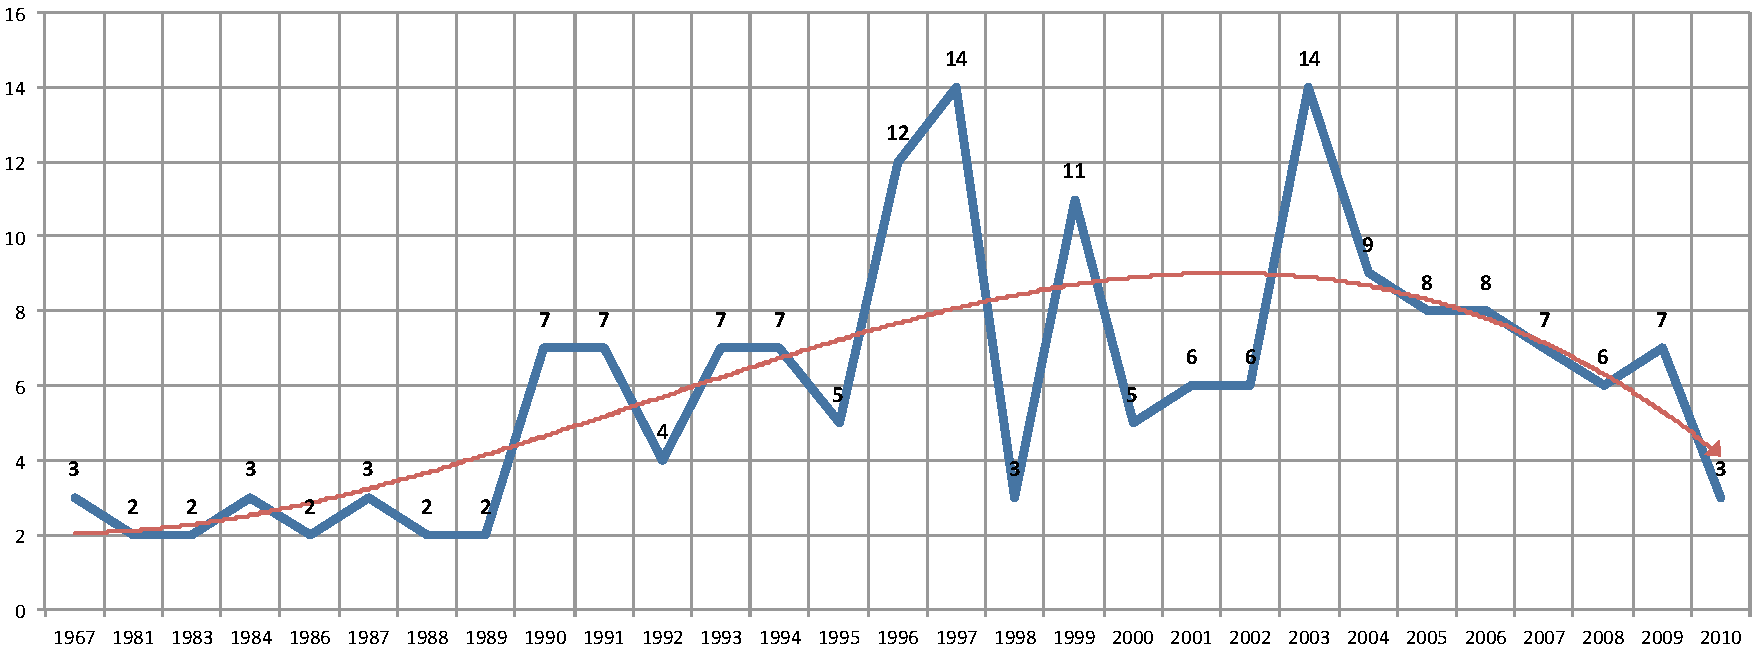
\includegraphics[width=1\textwidth]{figuras/abntex2-modelo-img-grafico.pdf}
\par\end{center}
\caption{Second side-by-side figure.\label{fig:side_b}}
\end{minipage}
\par\end{centering}

\legend{Fonte: Produzido pelos autores.}
\end{figure}

\section{Standard Tables}
\label{sec:tables}

For tables, place the caption above the tabular environment with the label nested inside. Using the \texttt{centering} block removes the unwanted vertical gap above the table.

\begin{table}[H]
\caption{A clean, native LyX table.\label{tab:results}}
\begin{centering}
\begin{tabular}{llc}
\toprule
Variable A & Variable B & Result \\
\midrule
Test 1 & Parameter X & 95\% \\
Test 2 & Parameter Y & 88\% \\
Test 3 & Parameter Z & 92\% \\
\bottomrule
\end{tabular}
\par\end{centering}

\legend{Fonte: Dados da pesquisa.}
\end{table}